\chapter{Exchange-Rate Fluctuations}\label{chp:fxf}
\hypertarget{fx}{}

%No extra lines here.
\textbf{Tools:} Arbitrage arguments.

\textbf{Key Words:} Real and nominal exchange rates; spot and forward exchange rates;
 purchasing power parity; covered/uncovered interest parity; the carry trade.

\textbf{Big Ideas:}
%\vspace{-0.1in}
\begin{itemize}
\item Exchange rates:  where sensible theory comes to die.
Meaning:  short-run movements in exchange rates are both hard to predict and hard to explain after the fact.
\item Purchasing power parity relates the relative price of goods across countries to exchange rates.
\item Interest rate parity (covered, uncovered) relates interest rates to exchange rates.
\item The empirical performance of purchasing power parity and uncovered interest parity is poor.
\end{itemize}

\rule{\textwidth}{1pt}

Exchange rates
(prices of foreign currency)
are a central element of most international transactions.
When Heineken sells beer in the US, its euro profits depend on its euro costs of production,
its dollar revenues in the US, and the dollar-euro exchange rate.
When a Tokyo resident purchases a dollar-denominated asset,
her return (in yen) depends on the asset's dollar yield
and the change in the dollar-yen exchange rate.
Exchange rates, then, are an essential component  of virtually all
international transactions.
%The essential role of the exchange rate is true of virtually
%all international transactions.

Nevertheless, countries in which exchange rates are determined
in open markets find that
short-term fluctuations are substantial, largely unpredictable,
and hard to explain after the fact.
That's been horribly disappointing to those of us who would like to
understand them better, but it's a fact of life.
From a business perspective, they're a source of random noise.
Heineken profits, for example, vary with the dollar-euro rate,
even if the underlying business doesn't change.

What follows is a summary of what we know.


\section{Terminology}

There is a lot  of jargon associated with this subject.
You'll run across references to:
%
\begin{itemize}

\item \textbf{Exchange-rate conventions.  \index{exchange rate!conventions}}
%
We typically express exchange rates as local currency prices of
one unit of foreign currency. \index{exchange rate}
In the US, we might refer to the dollar price of one euro.
In currency markets, the conventions vary
(every currency pair has its own),
but we'll try to stick with this one.
It has the somewhat strange feature that
an increase in the exchange rate is a decline in the relative value of the home currency.
Of course, it's also an increase in the value of the foreign currency.
As a rule of thumb, remember that we quote prices in dollars
(or whatever our local currency is).

\item \textbf{Exchange-rate changes.}
Changes in exchange rates also have their own names.
For a flexible exchange rate,
we refer to a decrease in the value of a currency as a
{\it depreciation\index{exchange rate!depreciation} \/} and an increase as an {\it appreciation\/}. \index{exchange rate!appreciation}
For a fixed exchange rate, where the changes reflect policy,\index{exchange rate regime!fixed exchange rate}
the analogous terms are {\it devaluation \index{exchange rate!devaluation}
 \/} and {\it revaluation  \index{exchange rate!revaluation}
 \/}.

\item \textbf{Real exchange rates. \index{exchange rate!real}}
You'll see this term, too, but what does it mean?
(What's an \emph{imaginary} exchange rate?)
A nominal exchange rate is the relative price of two currencies:
the number of units of currency A needed to buy one unit
of currency B.
The real exchange rate is the relative price of a commodity or
a basket of goods.
If $P$ is the US CPI in dollars, $P^*$ is the European CPI in euros,
and $e$ is the dollar price of one euro (the {\it nominal} exchange rate), then the (CPI-based) {\it real exchange rate\/} between the US and the Euro Zone is
\begin{eqnarray*}
    \mbox{\it RER\/}  &=& e P^* /P ,
\end{eqnarray*}
the ratio of the price of EU goods to US goods,
with both expressed in the same units (here, dollars).
We use an asterisk here and below to denote a foreign value.


\item \textbf{Parity relations.}
We generally think that trade (``arbitrage'')
will tend to reduce differences in prices and returns across countries.
Parity relations are based on the assumption that differences are
eliminated altogether.  It's an extreme assumption, to be sure,
but a useful benchmark.
{\it Purchasing power parity \index{purchasing power parity (PPP)} \/} is the theory that prices of baskets of goods are equal across countries:  $P = e P^* $
(or $\mbox{\it RER\/} = 1$).
This works for some specific goods (think of gold),
but anyone who takes a vacation abroad realizes that it is,
at best, a crude approximation for
broad categories of goods (hotels, restaurant meals, or the CPI).
{\it Interest rate parity \index{interest rate parity} \/} is the assumption that expected returns are equal
for comparable investments in different currencies --- think of US and Japanese treasury bills, or dollar- and yen-denominated eurocurrency deposits at major banks.
Despite the globalization of financial markets,
this doesn't work that well either.
% ?? covered ? uncovered?
%The carry trade is devoted to exploiting differences
%in expected returns across currencies.

\end{itemize}
%
We'll see each of these in action shortly.


\section{Properties of exchange rates}

Flexible exchange rates move around --- a lot.
The standard deviation of annual rates of change of currency prices
is ten to 12 percent for major currencies, more for emerging markets.
That's less than the standard deviation of equity returns
(the return on the S\&P 500 index has an annual standard deviation of 16-18 percent)
but a significant source of risk.
With a standard deviation of 10 percent, and assuming that changes in currency prices are normally distributed,
there's a five-percent chance of seeing a one-year change greater than 20 percent
either up or down.
%(That's if we use the normal distribution.
%Since currencies have fat tails, it's really a little worse than that.)

%Even worse, these changes are largely unpredictable.

You can get a sense of recent dollar movements from
Figure~\ref{fig:exch_rates},
which plots the price of one dollar expressed in Australian dollars,
British pounds, euros, yen, and yuan/renminbi, respectively.
(Inverses of dollar exchange rates, in other words.)
They are constructed as indexes, with the January 2001 values
set equal to 100.
You can see that the dollar-euro rate fluctuates quite a bit;
over the last five years, it's ranged from 70 to 110.
This reflects, to a large extent, the approaches taken by
the US and the European central banks\index{central bank}:
They let their currencies float freely.
The yen and the Australian dollar
are similar.
The renminbi, however, is fixed (or close to it)
by the Chinese central bank \index{central bank} at a value of about eight yuan per dollar.
%Fixed exchange rates are fairly common among developing countries.
More on this in the next chapter.

%
\begin{figure}[!ht]
    \caption{The US dollar against other major currencies.}
    \label{fig:exch_rates}
    \centering
    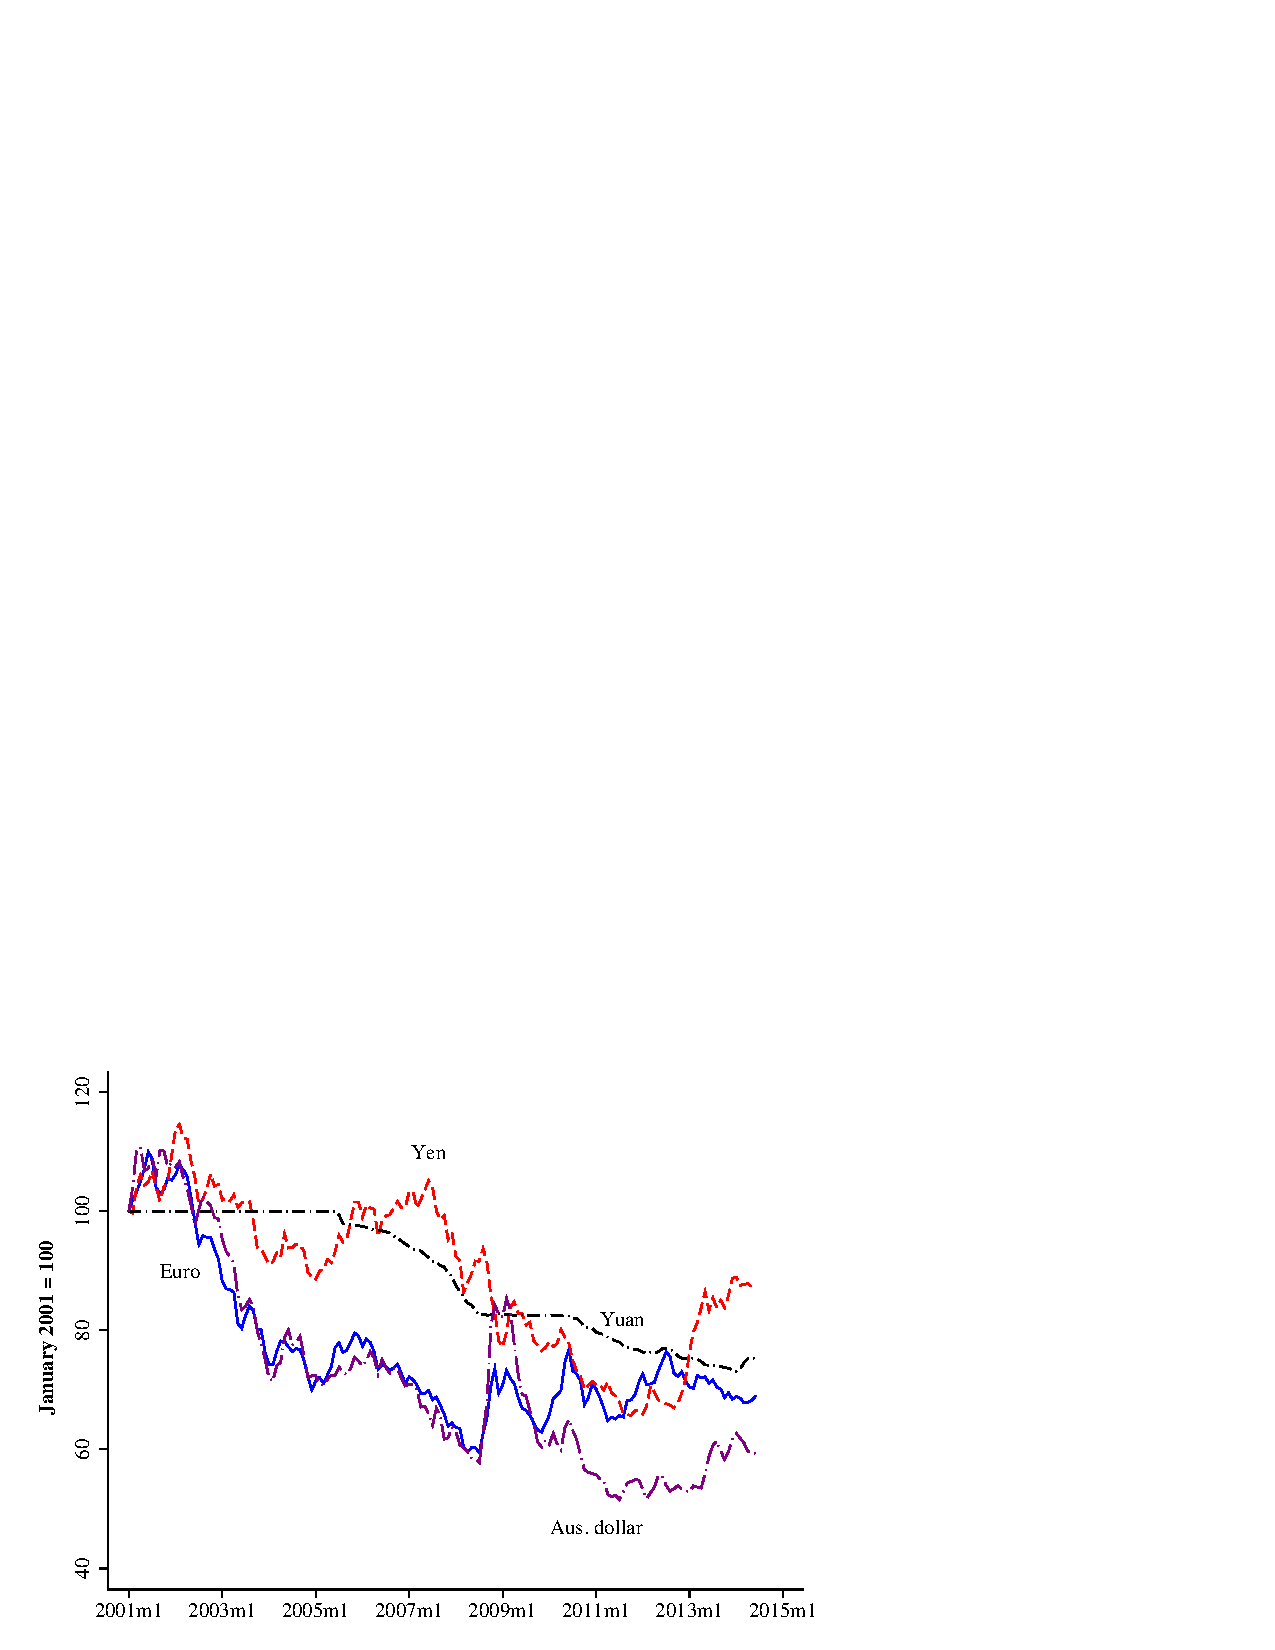
\includegraphics[width=0.8\textwidth]{\figpath Figures/exchange.pdf}
\end{figure}
%


\section{Purchasing-power parity \index{purchasing power parity (PPP)}
}

So we've seen that exchange rates move around.
But can we say anything about why?
We can't say much about short-term movements,
but here's a theory that gives us a long-term anchor
for the real exchange rate.
It's a helpful benchmark.

The idea is to compare prices of goods.
Suppose that exchange rates adjusted to equate prices across countries.
The logic is arbitrage:  If a good is cheaper in one
country than in another, then people would buy in the cheap country
and sell in the other, taking a profit along the way.
This process will tend to eliminate the difference in prices,
either through changes in the exchange rate or in the prices themselves.

Consider wine.
Suppose that a bottle of (some specific) wine costs $p=26$ dollars in New York,
and $p^*=20$ euros in Paris.
Are the prices the same?
If the exchange rate is $e=1.3$ dollars per euro,
then the New York and Paris prices are the same once we express them
in the same units.
More generally, we might say that
\begin{eqnarray*}
    p &=& e p^* .
\end{eqnarray*}
We refer to this relation as the {\it law of one price \index{law of one price} \/}:
that a product should sell for the same price in two locations.
An even better example might be gold,
which sells for pretty much the same price in
New York, London, and Tokyo.

If the law of one price works for some products,
there are many more for which restrictions on
trade (tariffs or quotas), transportation costs,
or other ``frictions'' prevent arbitrage.
Agricultural products, for example, are protected in many countries,
leading to substantial differences across countries
in the prices of such basic commodities as rice, wheat, and sugar.
Cement faces substantial shipping costs, even within countries.
Many services (haircuts, dry cleaning, medical and legal services)
are inherently difficult to trade,
and often protected by regulation, as well.

{\it The Economist\/}, with its usual flair for combining insight
with entertainment, computes dollar prices of the Big Mac around the
world.
The idea is that it's the same product everywhere, so differences
in prices reflect deviations from the law of one price.
In July 2014, Big Mac prices were \$4.80 in the US,
\$4.95 in the Euro Zone, \$3.64 in Japan, \$2.57 in Argentina,
and \$2.73 in China. These price differences vary
widely over time. For example, In January 2006, Big Mac prices  were \$3.15 in the US,
\$3.55 in the Euro Zone, \$2.19 in Japan, \$2.50 in Argentina,
and \$2.45 in China. Perhaps it's no surprise that the law of one price doesn't hold --- you can imagine the mess involved in trying to arbitrage price
differences.
But it's a good illustration of international price differences
more generally.


Despite such modest encouragement,
the first-cut theory of exchange rates is based on an application of
law-of-one-price logic to broad baskets of goods.
The so-called theory of purchasing power parity (PPP)
is that local and foreign price indexes ($P$ and $P^*$, say)
are linked through the exchange rate:  $ P \approx e P^* $ or
\begin{eqnarray}
    \mbox{\it RER\/} &=& eP^* /P \;\;\approx\;\; 1.
    \label{eq:ppp}
\end{eqnarray}
The approximation symbol suggests that we don't expect this to be perfect.
In the most common applications, the price indexes are CPIs
(consumer price indexes\index{price index!consumer price index (CPI)}),
and we refer to the measure of the real exchange rate as CPI-based.
If this doesn't work for specific goods, why might we expect it to hold
for average prices of goods?
One reason is that, for any pair of countries,
we might see as many products that are ``overpriced"
as there are products that are ``underpriced."
When we average, these deviations could offset each other, but,
in fact, they don't. If prices of some goods are cheaper abroad, then prices
of other goods tend to be, too.

What limited success we have comes in the long run.
As an empirical matter,
deviations from PPP tend to average out over time.
Sometimes prices are higher in Paris, sometimes higher in New York,
but, on average, prices are roughly comparable.
Prices are lower, on average, in countries with lower GDP per capita, but here, too, large fluctuations in the real exchange rate tend to disappear
with time.
How much time do we need for this to work?
At least several years.
If you're thinking of going to Paris next month,
there's little reason to expect that we'll be closer to PPP by then.
Maybe we will, maybe we won't; it's a tossup.


Real exchange rates computed this way are often used to judge whether
a currency's price is reasonable.
If the prices are lower at home than abroad ($\mbox{\it RER\/} > 1$),
we say the (home) currency is {\it undervalued\/}.
If prices are higher at home ($\mbox{\it RER\/} < 1$),
we say the currency is {\it overvalued\/}.
Over- and under-valued here means relative to our theory of PPP.
We can do the same thing with the Big Mac index.
We saw earlier that Big Macs were cheaper in China than in the US, so we might say that the dollar is overvalued relative to the yuan. Over time, we might expect most of these ``misvaluations'' to decline.
Experience suggests, however, that any such adjustment will take many years.
Our best estimates are that about half the difference from PPP will disappear
in five years. We can do the same thing with CPIs, with one difference: Since CPI are indexes, we don't know the absolute prices. The standard approach is to find the mean value of the real exchange rate
(or its logarithm) and judge under- or overvaluation by comparing the
real exchange rate to its mean, rather than one.


\section{Depreciation and inflation}

We can express the same theory in growth rates,
with the result that the change in the exchange rate
(the depreciation \index{exchange rate!depreciation} of the currency)
should equal the difference in the two inflation rates.
Simply put, if one country has a higher inflation rate than another,
then we would expect its currency to fall in value
by the difference.
That's not true over short periods of time,
but it's reasonable guide over longer periods of time.
Countries with high inflation rates find
that their currencies fall in value as a result.

Here's how that works.
The PPP relation  equation (\ref{eq:ppp}), implies that
\begin{eqnarray*}
    e_t &=& P_t/P_t^* .
\end{eqnarray*}
(Feel free to put $\approx$ here if you prefer.)
If we take (natural) logs of both sides, we have
\begin{eqnarray*}
    \ln e_t &=& \ln P_t - \ln P_t^* .
\end{eqnarray*}
If we take the same equation at two different dates,
we have
\begin{eqnarray*}
    \ln e_{t+1}-\ln e_{t} &=&
        (\ln P_{t+1}-\ln P_{t}) - (\ln P^{*}_{t+1}-\ln P^{*}_{t}) \\
                &=& \pi_{t+1} - \pi^*_{t+1} .
\end{eqnarray*}
In words:  The depreciation rate equals the difference in the inflation rates.
It's simply PPP in growth rates.


Does this work?
It's pretty good for long-run averages (five to ten years or more),
but like everything we know about exchange rates,
not very useful for short-term movements outside very
very-high-inflation situations.

\begin{figure}[ht]
    \caption{Venezuelan depreciation and inflation differential.}
    \label{fig:venezuela}
    \centering
    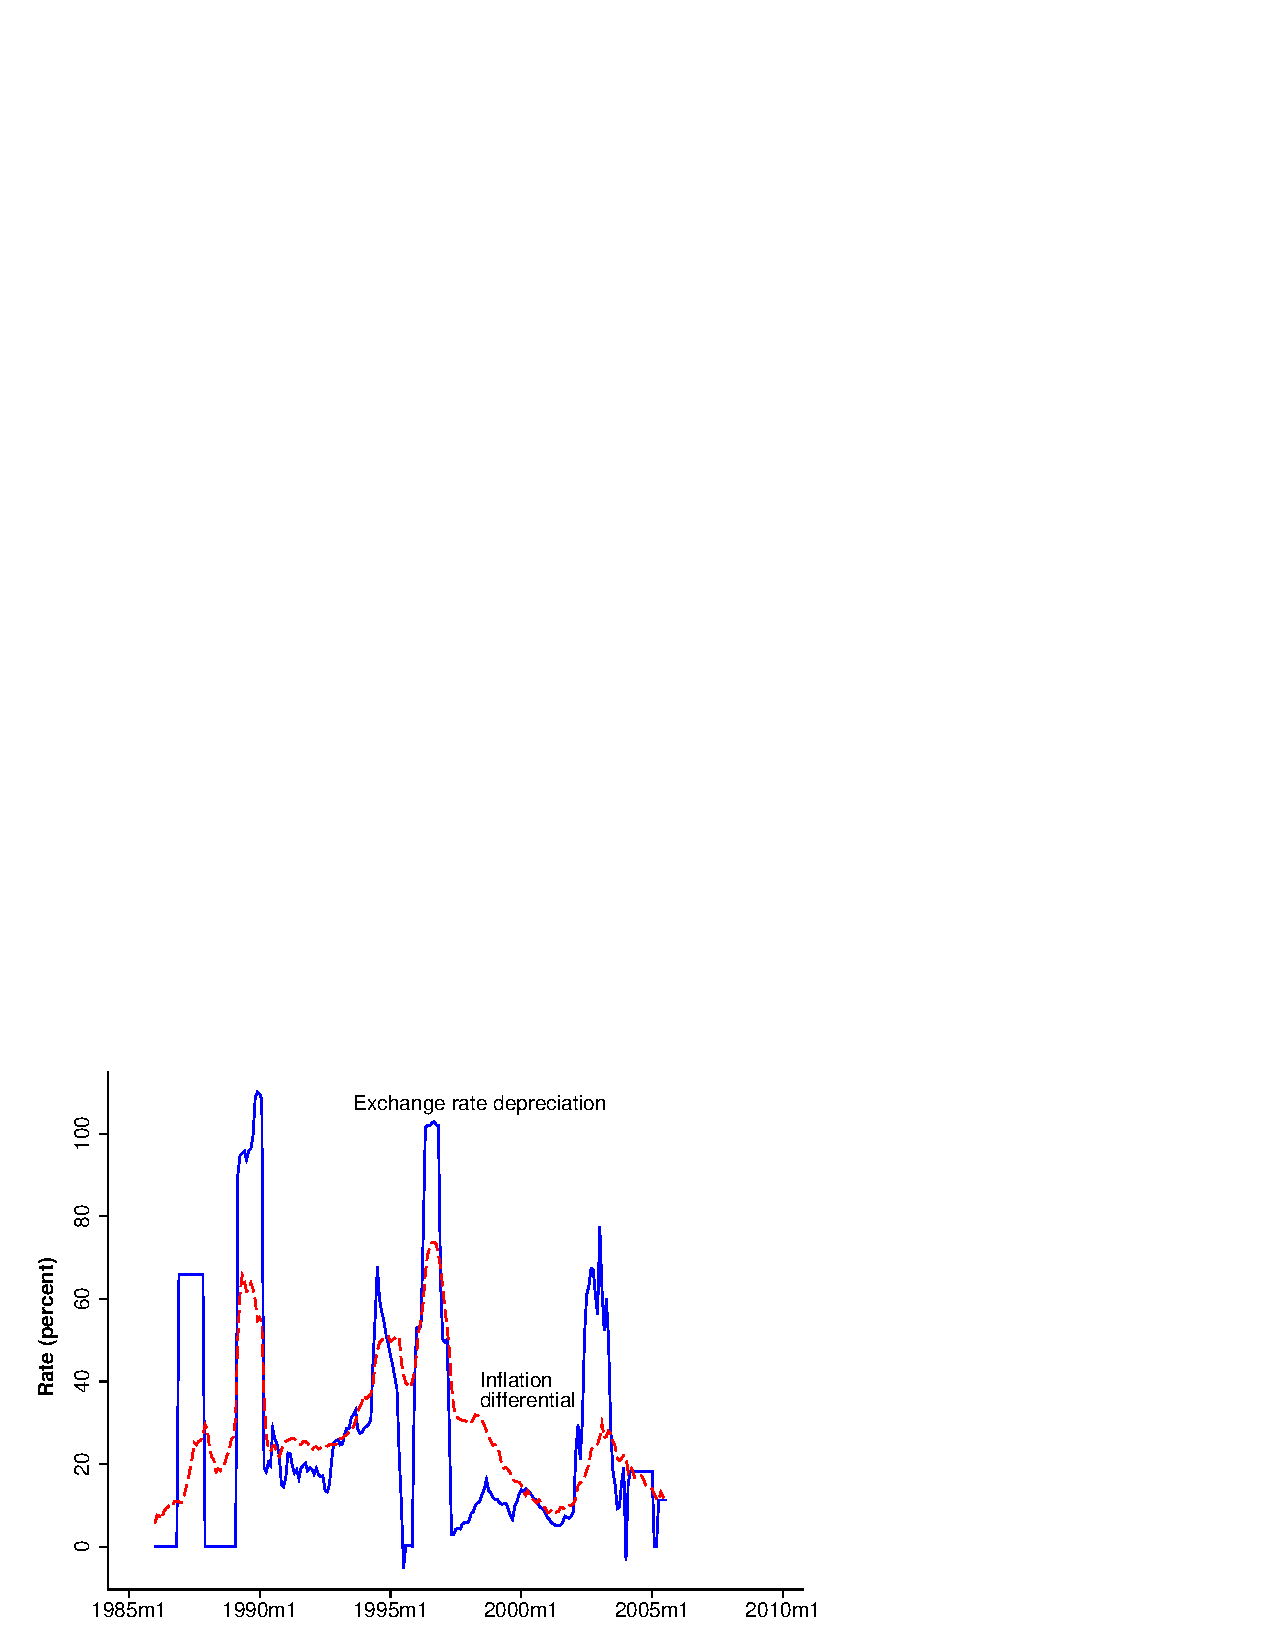
\includegraphics[width=0.8\textwidth]{\figpath Figures/venezuela.pdf}
\end{figure}

By way of example, consider the exchange rate between the Venezuelan
Bolivar and the US dollar. Between January 1985 and January 2006,
Venezuela's average annual inflation rate was 30 percent, as opposed to
the US's 2.9 percent. In the same period, the Bolivar
depreciated at the average yearly rate of 27.9 percent, i.e. only .8 percent
more than implied by the PPP condition. In the short run, however,
deviations from PPP are the norm.
Figure~\ref{fig:venezuela} shows that this has definitely been the
case for the Bolivar: There have been plenty of periods in which
exchange-rate depreciation did not closely track the inflation
differential with the United States. In some instances, in
particular in the late 1980s, the deviations were due to the central
bank's attempt to keep the exchange rate constant.
In other cases (the early 1990s, for example), the deviations
probably had nothing to do with central bank \index{central bank} interventions.

%
In developed countries, it's not unusual to see deviations of
the real exchange rate from one of 30-40 percent in either direction.
Figure~\ref{fig:us_euro} shows this for the dollar-euro.
\begin{figure}[ht]
    \caption{Dollar versus euro and inflation differential.}
    \label{fig:us_euro}
    \centering
    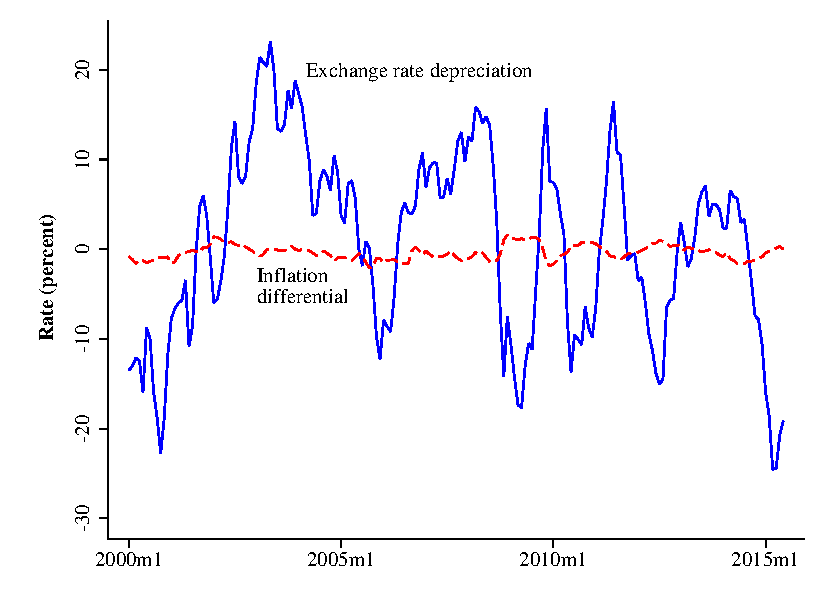
\includegraphics[width=0.8\textwidth]{\figpath Figures/us_euro.pdf}
\end{figure}
%
This picture is typical of developed countries: Inflation differentials are relatively small,
so changes in the real and nominal exchange rates are almost equal.
These deviations from PPP tend to disappear with time,
but, as we saw earlier, they go away slowly.


\section{Interest rate parity and the carry trade \index{interest rate parity}}

%  ?? change
%  interest diff and uip
%  carry trade and predictions

Exchange rates also play a role in interest rate differences across
countries. In June 2004, for example, three-month eurodollar deposits
paid interest rates of 1.40 percent in US dollars, 4.78 percent in British
pounds, 5.48 percent in Australian dollars, and 2.12 percent in euros. If
international capital markets are so closely connected, why do we see
such differences?  The answer is that these returns are
expressed in different currencies, so they're not directly comparable.\index{interest rate|(textbf}

Let's think about how prices of currencies show up in interest rate
differentials. We'll start with a relation called {\em covered
interest parity},  \index{interest rate parity!covered interest parity}
which says that interest rates denominated in
different currencies are the same once you ``cover'' yourself
against possible currency changes.  The argument follows the
standard logic of arbitrage used endlessly in finance.  Let's
compare two equivalent strategies for investing one US dollar for three
months. The first strategy is to invest one dollar in a three-month
eurodollar deposit (with the stress on ``dollar''). After three
months, that leaves us with $(1+i/4)$  dollars, where $i$ is the
dollar rate of interest expressed as an annual rate.

What if we invested one dollar in euro-denominated instruments? Here
we need several steps to express the return in dollars and make it
comparable to the first strategy. Step one is to convert the dollar
to euros, leaving us with $1/e$ euros
($e$ is the spot exchange rate --- the dollar price of one euro).
Step two is to invest this money
in a three-month euro deposit, earning the annualized rate of return
$i^{*}$. That leaves us with $(1+i^{*}/4)/e$ euros after three
months. We could convert it at the spot rate prevailing three months
from now, but that exposes us to the risk that the euro will fall.
An alternative is to sell euros forward at price $f$. In three
months, we will have $(1+i^{*}/4)/e$ euros that we want to convert
back to dollars. With a three-month forward contract, we arrange now
to convert them at the forward rate $f$ expressed, like $e$, as
dollars per euro. This strategy leaves us with $(1+i^{*}/4)f/e$
dollars after three months.

Thus, we have two relatively riskless  strategies, one yielding
$(1+i/4)$, the other yielding $(1+i^{*}/4)f/e$. Which is better?
Well, if either strategy had a higher payoff, you could short one
and go long on the other, earning extra interest with no risk.
Arbitrage will tend to drive the two together:
\begin{equation}
                            (1+i/4) \;\;=\;\; (1+i^{*}/4)f/e.
                            \label{eq:cip}
\end{equation}
We call (\ref{eq:cip}) {\it covered interest parity\/}.
Currency traders assure us that covered interest parity
is an extremely good approximation in the data, except in extreme periods of liquidity,
such as a financial crisis. The only difference between the left and right sides is a bid-ask spread,
which averages less than 0.05 percent for major currencies.


A related issue is whether international differences
in interest rates reflect differences in expected depreciation rates.
Does the high rate on Aussie dollars (AUD)
reflect the market's assessment that
the AUD will fall in value relative to (say) the euro?
To see how this works, suppose
that we converted the proceeds of our foreign investment
back to local currency at the exchange rate prevailing
in three months.  Our return would then be
\[
                            (1+i^{*}/4) e_{3}/e ,
\]
where $e_3$ is the spot exchange rate three months in the future.
This investment is risky, since we don't know what the
future exchange rate will be, but we might expect
it to have a similar expected return to a local investment.
That is,
\begin{equation}
          (1+i/4) \;\;=\;\; (1+i^{*}/4) E (e_{3})/e ,
          \label{eq:uip}
\end{equation}
where $E(e_3)$ is our current expectation
of the exchange rate in three months.
This relation is an application of the expectations hypothesis to
currency prices (the forward rate equals the expected future spot rate)
that is commonly referred to as {\it uncovered interest parity\/}. \index{interest rate parity!uncovered interest parity}


In fact, uncovered interest rate parity doesn't work.
It implies that high-interest-rate currencies depreciate,
when, in fact, they appreciate (increase in value) on average,
making them potentially good (if risky) investments.
If $i>i^*$, we invest at home.  If $i<i^*$, we invest abroad,
expecting to pocket not only the higher interest rate but
an appreciation of the currency ($e_3>e$).
That's the essence of what is called the ``carry trade.''
Why this investment opportunity persists remains something of a mystery to
academics and investors alike.

Two fine points:  (i)~This feature of the data does not apply to
the currencies of developing countries, where higher interest rates
typically do imply future depreciation.
That is, uncovered interest parity   works better here.
(ii) In developed countries, forecasts of exchange-rate changes based on interest differentials have an $R^2$ of 0.05 or less.
That's still useful for investment purposes,
but leaves most of the variance of exchange-rate changes unexplained.


\section{Predicting exchange rates}

Let's summarize what we've learned about movements in exchange rates:
%
\begin{itemize}
\item PPP works reasonably well over long periods of time,
but has little empirical content over periods of less than a few years,
and virtually none over periods under a year.

\item Interest rate differentials have some forecasting power,
with high-interest-rate currency increasing in value, on average,
but they leave most of the variance of exchange-rate movements
 unexplained.
\end{itemize}
%
Can we do better than this?
A little, but probably no more than that.
It's extremely hard to forecast exchange rates better than
a 50-50 bet on up or down.
Interest differentials do a little better, but only a little. We may be able to do better still
using more complex theory or personal judgment about policy,
but years of failure suggest that
it's very hard to beat a random walk consistently.



\section*{Executive summary}

%\setlength{\leftmargini}{.5\oldleftmargini}
\begin{enumerate}
\item In the long run, exchange rates tend to
equalize prices of products across countries (PPP).

\item In the short run, exchange-rate movements are large
and unpredictable.
\end{enumerate}
%\setlength{\leftmargini}{\oldleftmargini}


\section*{Review questions}

%\setlength{\leftmargini}{.5\oldleftmargini}
\begin{enumerate}
\item Purchasing power parity for Big Macs.
The Economist reports the following data for
local prices of Big Macs and US dollars in July 2011:
%
\begin{center}
\begin{tabular}{lccc}
\toprule
        & Big Mac Price  &  Exchange Rate    \\
        &(Local Currency)&(LCUs per Dollar)   \\
        &  (A)  &  (B) \\
\midrule
Argentina       &  20.0  &  4.13  \\
Brazil          &  9.50  &  1.54 \\
India           &  84.0  &  44.4   \\
United States   &  4.07  &  1.00   \\
\bottomrule
\end{tabular}
\end{center}
LCUs are ``local currency units.''


\begin{enumerate}
\item What is the dollar price of a Big Mac in each of these locations?
\item In what ways is the ratio of USD Big Mac prices similar to the real exchange rate?
\item What exchange rates for the first three currencies would
equate the dollar prices of Big Macs in other countries to the US price?
How is this related to PPP?
\item How much are the first three currencies over or undervalued
relative to the US dollar?
\end{enumerate}

Answer.  The calculations are summarized in
%
{\small
\begin{center}
\begin{tabular}{lccc}
\toprule
        & Big Mac   &  Big Mac  & Overvaluation\\
        &  (USD)&   (Ratio) &  (percent)\\
        & (C) & (D) & (E)  \\
\midrule
Argentina       &  4.84 &  4.91  &  19\\
Brazil          &  6.17 &  2.33  & 51\\
India           &  1.89 &  20.64 & $-53$\\
United States   &  4.07 &  1.00  & 0.0\\
\bottomrule
\end{tabular}
\end{center}
}

\begin{enumerate}
\item Dollar prices of Big Macs are reported above as column (C),
computed as (A)/(B).

\item The relative price of Big Macs is like a real exchange rate.
The real exchange rate is the ratio of prices converted to a common currency:
\begin{eqnarray*}
    \mbox{\it RER\/}  &=&  eP^*/P .
\end{eqnarray*}
Usually we use prices indexes for $P$ and $P^*$, here we use prices of Big Macs.

\item Mathematically, we set $\RER$ equal to one (the PPP condition)
and solve for $e = P/P^*$.
In the table, we computed this as the ratio of entries on column (A) to the US
entry in the same column.
That gives us a PPP benchmark for what the exchange rate should be.

\item If we compare our calculation of the PPP exchange rate in (c) to the actual,
we can see how far off we are.
In the table, we compute ``overvaluation'' as the percentage difference between
true exchange rates and our PPP calculation:  {\tt 100*[(D)/(B)-1]}.
We see that the Brazilian real is overvalued (Big Macs are expensive there)
and the Indian rupee is undervalued (Big Macs are cheap there).
\end{enumerate}

\item Forecasting the euro.
Suppose the euro is ``overvalued'' in PPP terms relative to the
dollar (goods are more expensive in Europe) and Euro Zone short-term interest rates
are slightly above US interest rates.
Given these facts, how would you expect the euro/dollar exchange rate to change over the next 6 months?  6 years?
How good is each of these informed guesses?

Answer.  Purchasing power parity is a long-run ``anchor'' for the
exchange rate:  if prices of goods and services in the Euro Zone
are higher than those in the US, when expressed in a common currency,
we'd expect the euro to fall in value relative to the dollar
--- eventually.
This is pretty much useless over a period as short as 6 months,
but has some content over 6 years.
More useful in the short-run is the interest differential.
Since the Euro interest rate is higher, we'd expect the euro to increase in value.
Neither works well:  an $R^2$ of 0.05 would be good over
periods of a few months.\index{interest rate|)}
\end{enumerate}
%\setlength{\leftmargini}{\oldleftmargini}


\section*{If you're looking for more}

\href{http://research.stlouisfed.org/fred2/}{FRED}
has exchange rates for many countries.
So does the
\href{http://www.federalreserve.gov/releases/h10/hist/}{Fed};
search:  ``fed exchange rates.''

The Economist's
\href{http://www.economist.com/content/big-mac-index}{Big Mac index}
(search: ``big mac index'')
is the center of a nice web site on exchange-rate data and issues.

Deutsche Bank's
%\href
%{http://www.deutsche-bank.de/presse/en/releases_761.shtml}
{\it Guide to Exchange-Rate Determination\/} is a terrific
summary of what we know about exchange rates from a
bond \index{bond} and currency trader's perspective.




\section*{Symbols and data used in this chapter}

\begin{table}[H]
\centering
\caption{Symbol table.}
\begin{tabular*}{0.98\textwidth}{l@{\extracolsep{\fill}}l}
\toprule
Symbol & Definition \\
\midrule
$e$      &Spot exchange rate = home currency price of foreign currency\\
$f$      &Forward exchange rate \\
$P$     &Domestic price level\\
$P^*$    &Foreign  price level\\
$\mbox{\it RER\/}$  & Real exchange rate $= eP^*/P$  \\
$\pi$     &Domestic inflation\\
$\pi^*$     &Foreign inflation\\
$i$     &Domestic nominal interest rate \\
$i^*$    &Foreign nominal interest rate \\
${E}(x)$    &Expected value of a variable $x$\\
\bottomrule
\end{tabular*}
\end{table}

\begin{table}[htb]
\centering
\caption{Data table.}
\begin{tabular*}{0.98\textwidth}{l@{\extracolsep{\fill}}l}
\toprule
Variable & Source\\
\midrule
USD/euro exchange rate    &EXUSEU\\
Yuan/USD exchange rate    &EXCHUS\\
Yen/USD exchange rate    &EXJPUS\\
USD/UK pound exchange rate    &EXUSUK\\
USD/AUD exchange rate    &EXUSAL\\
Venezuela/USD exchange rate    &EXVZUS\\
Real trade-weighted USD index (broad)    &TWEXBPA\\
US consumer price index
    &CPIAUCSL\\
Euro area harmonized consumer price index
     &CP0000EZCCM086NEST\\
\bottomrule
\addlinespace
\end{tabular*}
\begin{minipage}{0.98\textwidth}
\footnotesize{To retrieve the data online, add the identifier from the source column to \url{http://research.stlouisfed.org/fred2/series/}.  For example, to retrieve the dollar-euro exchange rate, point your browser to \url{http://research.stlouisfed.org/fred2/series/EXUSEU}}
\end{minipage}
\end{table}
